\documentclass[tikz, border=3pt]{standalone}
\usepackage{tikz}
\usetikzlibrary{decorations.pathreplacing,patterns, arrows, arrows.meta, shapes}
\definecolor{greengreen}{rgb}{0.0, 0.42, 0.24}
%%%%%%%%%%%%%%%%%%%%%%%%%%%%%%%%%%%%%%%%%%%%%%%%%%%%%%%%%%%%%%%%%
\begin{document}
%%%%%%%%%%%%%%%%%%%%%%%%%%%%%%%%%%%%%%%%%%%%%%%%%%%%%%%%%%%%%%%%%
\tikzset{>={Latex[width=3mm,length=3mm]}}
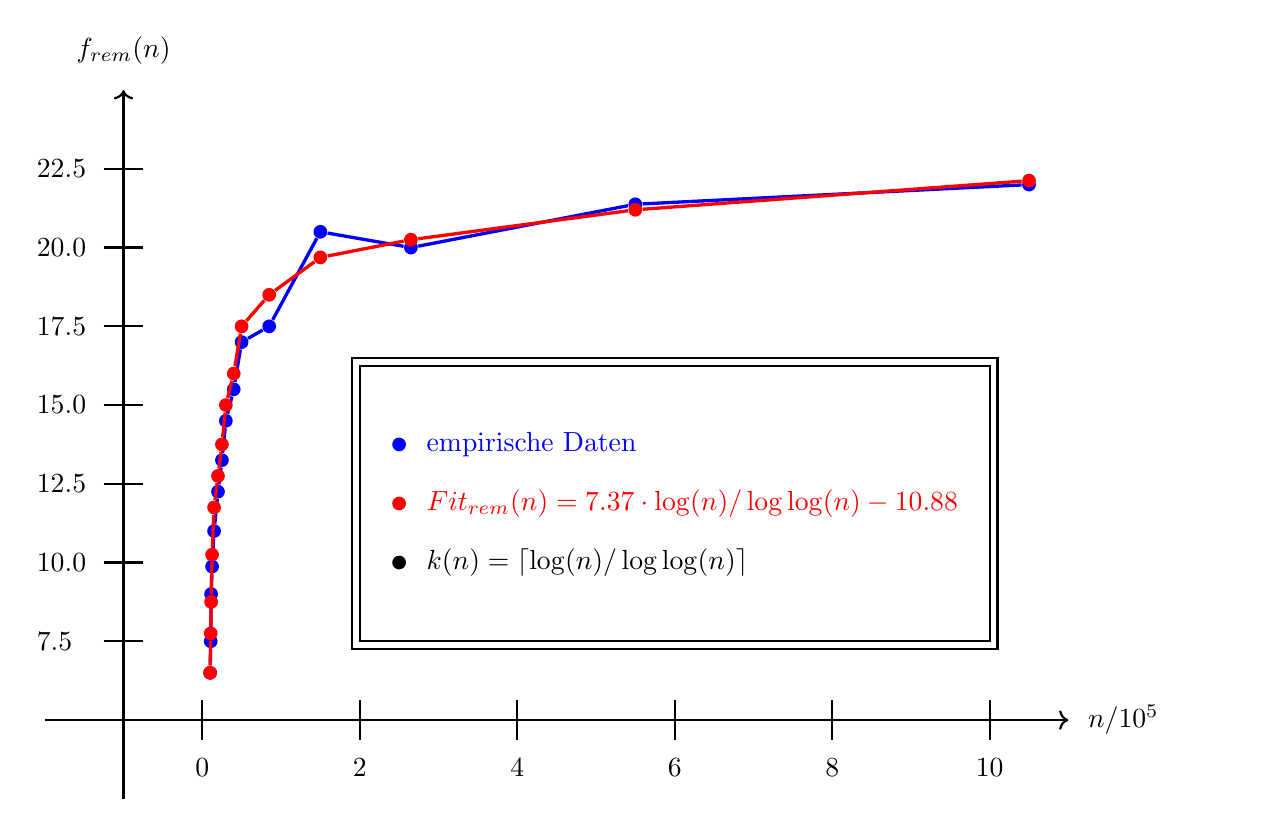
\begin{tikzpicture}[every node/.style={align=center, thick, scale=1},
red/.style={fill=red,circle,inner sep=0pt,scale = 0.5},
blue/.style={fill=blue,circle,inner sep=0pt,scale = 0.5},
black/.style={fill=black,circle,inner sep=0pt,scale = 0.5},
 text width = .35cm]
%================================================================
% Axis
% --------------------------------
% X-Axis
\draw[thick, ->] (-1,0) -- (12,0);
\node[thick, align=left, text width=2cm] at (13.25,0) {$n/10^5$};
\foreach \x in {1,3,5,7,9,11}
  \draw[thick] (\x,-0.25) -- (\x,0.25);
  \node[thick, align=center, text width=1cm] at (1,-0.6) {$0$};
\node[thick, align=center, text width=1cm] at (3,-0.6) {$2$};
\node[thick, align=center, text width=1cm] at (5,-0.6) {$4$};
\node[thick, align=center, text width=1cm] at (7,-0.6) {$6$};
\node[thick, align=center, text width=1cm] at (9,-0.6) {$8$};
\node[thick, align=center, text width=1cm] at (11,-0.6) {$10$};

% --------------------------------
% Y-Axis
\draw[thick, ->] (0,-1) -- (0,8);
\node[thick, align=center, text width=2cm] at (0,8.5) {$f_{rem}(n)$};
\foreach \y in {1,2,3,4,5,6,7}
  \draw[thick] (-0.25,\y) -- (0.25,\y);
\node[thick, align=left, text width=1cm] at (-0.6,1) {$7.5$};
\node[thick, align=left, text width=1cm] at (-0.6,2) {$10.0$};
\node[thick, align=left, text width=1cm] at (-0.6,3) {$12.5$};
\node[thick, align=left, text width=1cm] at (-0.6,4) {$15.0$};
\node[thick, align=left, text width=1cm] at (-0.6,5) {$17.5$};
\node[thick, align=left, text width=1cm] at (-0.6,6) {$20.0$};
\node[thick, align=left, text width=1cm] at (-0.6,7) {$22.5$};

%================================================================
% Data
\node[style=blue] (d1) at (1.1,0.6) {};
\node[style=blue] (d2) at (1.1075,1) {};
\node[style=blue] (d3) at (1.1125,1.6) {};
\node[style=blue] (d4) at (1.125,1.95) {};
\node[style=blue] (d5) at (1.15,2.4) {};
\node[style=blue] (d6) at (1.2,2.9) {};
\node[style=blue] (d7) at (1.25,3.3) {};
\node[style=blue] (d8) at (1.3,3.8) {};
\node[style=blue] (d9) at (1.4,4.2) {};
\node[style=blue] (d10) at (1.5,4.8) {};
\node[style=blue] (d11) at (1.85,5) {};
\node[style=blue] (d12) at (2.5,6.2) {};
\node[style=blue] (d13) at (3.65,6.0) {};
\node[style=blue] (d14) at (6.5,6.55) {};
\node[style=blue] (d15) at (11.5,6.8) {};

\draw[very thick, color=blue] (d1) -- (d2) -- (d3) -- (d4) -- (d5) -- (d6) -- (d7) -- (d8) -- (d9) -- (d10) -- (d11) -- (d12) -- (d13) -- (d14) -- (d15);

%================================================================
% Fit
\node[style=red] (f1) at (1.1,0.6) {};
\node[style=red] (f2) at (1.1075,1.1) {};
\node[style=red] (f3) at (1.1125,1.5) {};
\node[style=red] (f4) at (1.125,2.1) {};
\node[style=red] (f5) at (1.15,2.7) {};
\node[style=red] (f6) at (1.2,3.1) {};
\node[style=red] (f7) at (1.25,3.5) {};
\node[style=red] (f8) at (1.3,4) {};
\node[style=red] (f9) at (1.4,4.4) {};
\node[style=red] (f10) at (1.5,5) {};
\node[style=red] (f11) at (1.85,5.4) {};
\node[style=red] (f12) at (2.5,5.875) {};
\node[style=red] (f13) at (3.65,6.1) {};
\node[style=red] (f14) at (6.5,6.48) {};
\node[style=red] (f15) at (11.5,6.85) {};

\draw[very thick, color=red] (f1) -- (f2) -- (f3) -- (f4) -- (f5) -- (f6) -- (f7) -- (f8) -- (f9) -- (f10) -- (f11) -- (f12) -- (f13) -- (f14) -- (f15);

%================================================================
% Legend
\draw[thick] (3,1) rectangle (11,4.5);
\draw[thick] (2.9,0.9) rectangle (11.1,4.6);

% Data
\node[style=blue] at (3.5,3.5) {};
\node[thick, color=blue, align=left, text width=7cm] at (7.35,3.5) {empirische Daten};

% Fit
\node[style=red] at (3.5,2.75) {};
\node[thick, color=red, align=left, text width=7cm] at (7.35,2.75) {$Fit_{rem}(n)=7.37\cdot\log(n)/\log\log(n) - 10.88$};

% k(n)
\node[style=black] at (3.5,2) {};
\node[thick, color=black, align=left, text width=7cm] at (7.35,2) {$k(n)=\lceil\log(n)/\log\log(n)\rceil$};


%================================================================
\end{tikzpicture}
%%%%%%%%%%%%%%%%%%%%%%%%%%%%%%%%%%%%%%%%%%%%%%%%%%%%%%%%%%%%%%%%%
\end{document}
%%%%%%%%%%%%%%%%%%%%%%%%%%%%%%%%%%%%%%%%%%%%%%%%%%%%%%%%%%%%%%%%%
